本章では ArchHDL での実行時間を評価し,Icarus Verilog, NC-Verilog, VCS での論理シミュレーションの実行時間と比較する.

\begin{table}[t]
 \caption{実行環境}
 \label{table:exec_env}
 \begin{center}
  \begin{tabular}{l|c|c} \hline
         &  Icarus Verilog, ArchHDL  &  NC-Verilog, VCS   \\ \hline
  OS     &  Ubuntu12.04             &  CentOS5.9        \\
  CPU    &  Core i7-3770K 3.50GHz   &  Core i7-3770K 3.50GHz  \\
  メモリ  &  $16\,\mathrm{GB}$       &  $16\,\mathrm{GB}$  \\ \hline
  \end{tabular}
 \end{center}
\end{table}

同じ仕様の 2 台の計算機を用いる.
一台は Icarus Verilog, ArchHDL の評価に用いる.もう一台は NC-Verilog, VCS の評価に用いる.
\tabref{table:exec_env} に実行環境をまとめる.
CPU,メモリなどのハードウェアの仕様は同一である.
一方ソフトウェアの制約により異なる OS を利用する.

異なる OS を用いる理由を述べる.
NC-Verilog と VCS は RedHat 系のみをサポートしている.
よって RedHat 系のディストリビューションである CentOS を用いる.
しかし CentOS5.9 に含まれる gcc のバージョンは 4.1.2 である.
\ref{ss:modeling}節で述べたように ArchHDL では C++11 のラムダ関数を用いて記述するため gcc のバージョンは 4.5 以上が必要である.
そこで Ubuntu12.04 を用いる.
Ubuntu12.04 に含まれる gcc のバージョンは 4.6.3 である.
Icarus Verilog はどちらのディストリビューションでも動作するが,今回は Ubuntu12.04 を用いる.
Ubuntu12.04 に含まれる Icarus Verilog のバージョンは 0.9.5 である.

評価では,マイクロベンチマークとして 2 つの回路,現実的なハードウェアのベンチマークとしてステンシル計算回路\cite{koba:stencil}を用いる.
Verilog HDL と ArchHDL のためのハードウェア記述の記述は手作業により記述した.
両ハードウェア記述の出力は同様になるように記述した.


\subsection{マイクロベンチマークによる評価}

マイクロベンチマークとしてカウンタ回路と XORSHIFT による乱数生成回路を用いる.

\begin{figure}[t]
 \lstinputlisting[language=c++]{src/xorshift_alg.cc}
 \caption{XORSHIFT 法に基づく乱数生成のアルゴリズム}
 \label{src:xorshift_alg}
\end{figure}

カウンタ回路とは \figref{src:counter} に示した 1 サイクルごとに 1 を足す回路である.
ハードウェアの規模を増やすためにカウンタの数を指定できるようにした.
XORSHIFT による乱数生成回路とはシフトと XOR 演算のみで構成できる XORSHIFT 法に基づく乱数生成器をハードウェア記述によって実装した回路である.
\figref{src:xorshift_alg} に XORSHIFT 法に基づく乱数生成のアルゴリズムを C 言語によって実装したものを示す.

\begin{figure}[t]
 \centering
 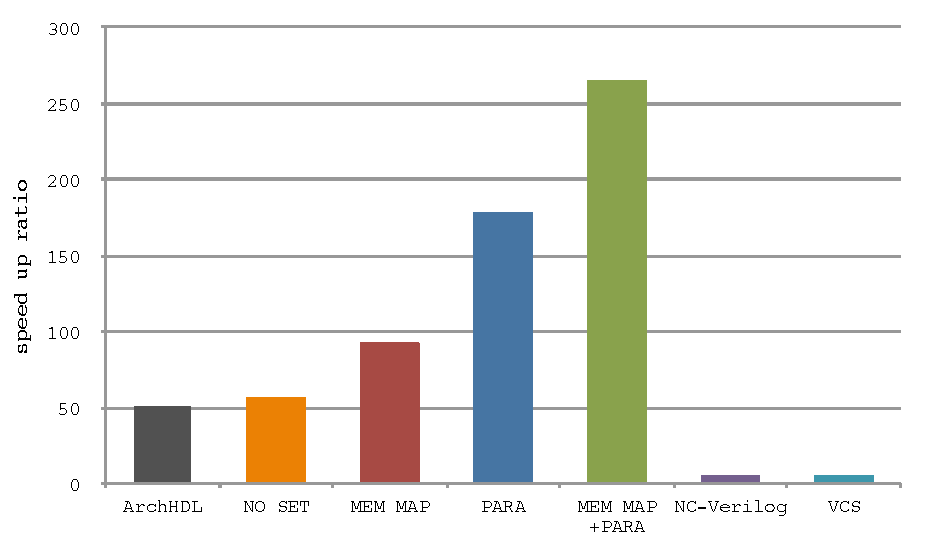
\includegraphics[clip,width=\linewidth]{counter_4096}
 \caption{4096 個のカウンタ回路の実行時間を Icarus Verilog と比較した速度向上比}
 \label{fig:counter4096}
\end{figure}

\figref{fig:counter4096} に 4096 個のカウンタ回路の実行時間を Icarus Verilog と比較した速度向上比を示す.
縦軸は Icarus Verilog での実行時間を 1 とした速度向上比を示している.

ArchHDL は商用の NC-Verilog, VCS と比較してもかなり高速である.
高速化手法と並列化を共に適用した場合と比べると ArchHDL は NC-Verilog の約 58.8 倍,VCS の約 56.7 倍高速である.

また今回提案している高速化手法は効果が出ている.
高速化手法と並列化を共に適用した ArchHDL のシミュレーションはオリジナルの ArchHDL より約 5.23 倍高速である.



\begin{figure}[t]
 \centering
 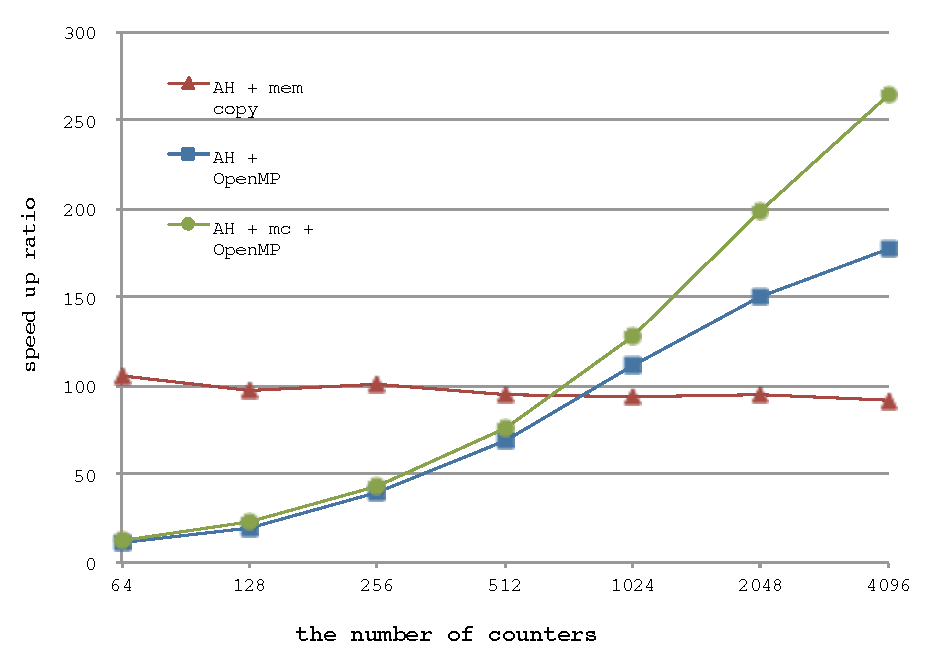
\includegraphics[clip,width=\linewidth]{counter_con}
 \caption{高速化手法を適用した ArchHDL と OpenMP を適用したカウンタ回路の実行時間を Icarus Verilog と比較した速度向上比}
 \label{fig:counter_con}
\end{figure}

\figref{fig:counter_con} に高速化手法を適用した ArchHDL と OpenMP を適用したカウンタ回路の実行時間を Icarus Verilog と比較した速度向上比を示す.
縦軸は Icarus Verilog での実行時間を 1 とした速度向上比を示している.
横軸はカウンタの個数である.

逐次実行は Icarus Verilog と比較して速度向上比はほぼ一定である.
並列化を行った場合はカウンタの個数が 1024 個を超えた所で逐次実行よりも高速になる.

カウンタの個数はハードウェアの規模とみなせるため,並列化が有効なのはある程度規模の大きい回路であると言える.

また \ref{sss:mem_copy} 節で述べた高速化手法は並列化を行った場合でも一貫して効果が出せている.

\begin{figure}[t]
 \centering
 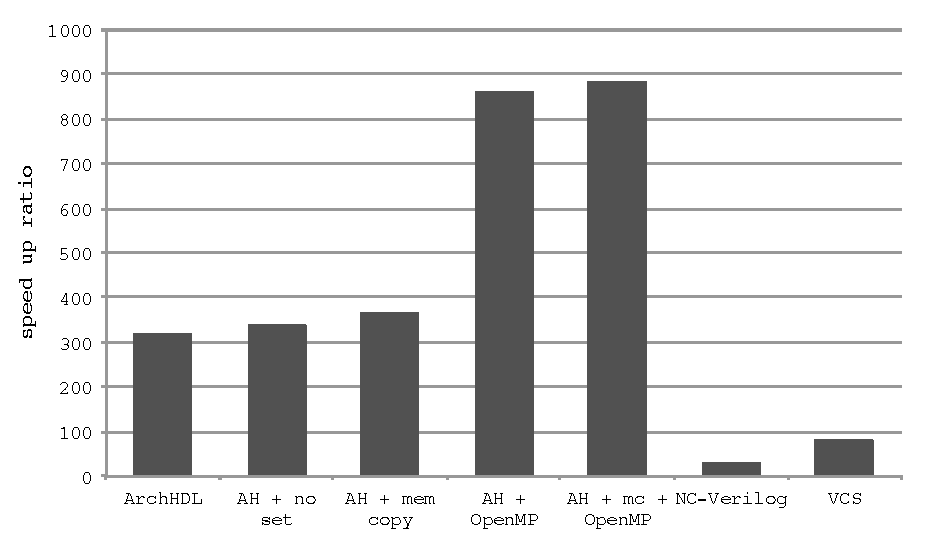
\includegraphics[clip,width=\linewidth]{xorshift}
 \caption{512 個の XORSHIFT による乱数生成器の実行時間を Icarus Verilog と比較した速度向上比}
 \label{fig:xorshift}
\end{figure}

\figref{fig:xorshift} は XORSHIFT による乱数生成器での実行時間を Icarus Verilog と比較した速度向上比である.
試行回数は 524,288 回である.初期値の異なる乱数生成器を 512 個用意している.

ArchHDL は商用の NC-Verilog, VCS と比較してもかなり高速である.
高速化手法と並列化を共に適用した場合と比べると ArchHDL は NC-Verilog の約 32.2 倍,VCS の約 11.3 倍高速である.

高速化手法と並列化を共に適用した ArchHDL のシミュレーションはオリジナルの ArchHDL より約 2.78 倍高速である.


\subsection{ステンシル計算回路による評価}

\if0

\begin{table}[t]
 \caption{ステンシル計算回路でのプロファイリング結果 1.1}
 \label{table:stencil_prof1.1}
 \begin{center}
  % \setlength{\tabcolsep}{3pt}
  \begin{tabular}{lr} \toprule
  関数名 & 実行時間に占める割合 (\%) \\ \midrule
  reg::Update() (合計) & 16.57 \\
  ArchHDL::Step() & 12.47 \\
  brk & 15.05 \\ \bottomrule
  \end{tabular}
 \end{center}
\end{table}

\fi

\begin{figure}[t]
 \centering
 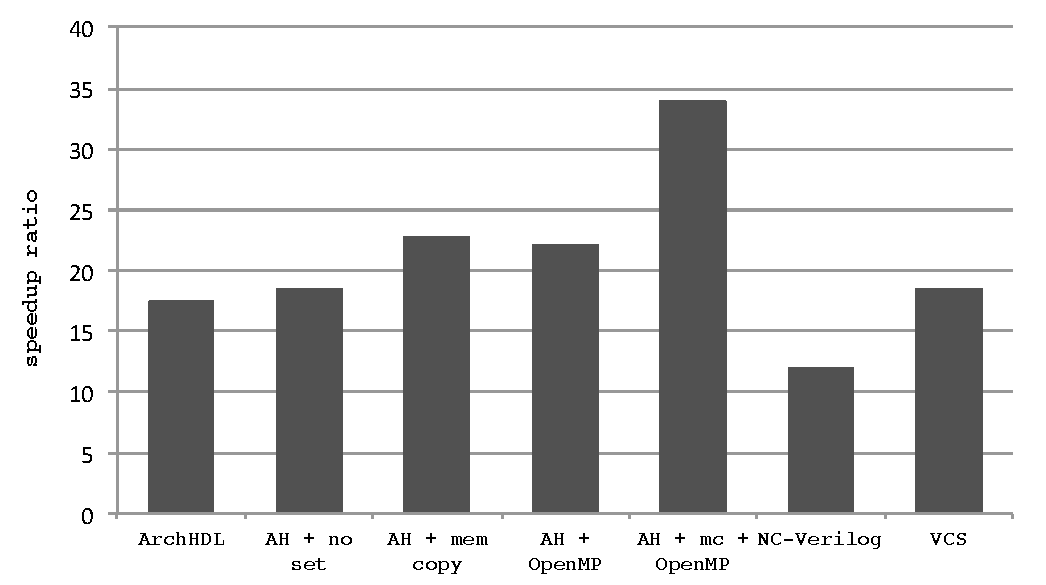
\includegraphics[clip,width=\linewidth]{stencil}
 \caption{ステンシル計算回路の Icarus Verilog と比較した実行時間の速度向上比}
 \label{fig:stencil}
\end{figure}

\figref{fig:stencil} はステンシル計算回路での実行結果である.

縦軸は Icarus Verilog と比較したそれぞれの速度向上比である.

OpenMP による並列化はスレッド数を 8 個にして計測している.

ステンシル計算回路の場合は Update() は 325,469,175 回呼ばれているのに対して,
reg の値が更新されるのは 320,323,415 回であり, reg の値に更新がないのは 5,145,760 回である.
つまり更新がないのは全体の約 $1.58\%$ 程度に過ぎない.
そのため \ref{sss:no_set} 節で述べたデータ変更の有無による条件分岐の除去を行った方が高速になる.

また Update() は 325,469,175 回呼ばれているのでこのメソッド呼び出しを減らし,
かつ代入をメモリーコピーにする \ref{sss:mem_copy} 節の逐次代入をメモリーコピーにする方が高速になっている.

また Module が 133 個,reg が 991 個存在する回路なので並列化の効果も大きい.

NC-Verilog は ArchHDL より高速でない.
VCS は ArchHDL と set\_ 変数なしの実装より高速であるが,メモリーコピーにする実装よりは高速でない.

高速化手法と並列化を共に適用した場合と比べると ArchHDL は VCS より約 1.83 倍高速である.




% \subsection{高速化の解析}
